% Sets up the document template, imports needed packages and other useful ones, and defines some useful commands

\usepackage[printonlyused]{acronym}
\usepackage{amsmath}
\usepackage{breqn}
\usepackage[blocks]{authblk}
\usepackage[backend=biber,sorting=none]{biblatex}
\usepackage[justification=justified,singlelinecheck=off,bf]{caption}
\usepackage{chngcntr}
\usepackage{changepage}
\usepackage[usenames,dvipsnames]{color}
\usepackage{enumerate}
\usepackage{enumitem}
\usepackage{fancyhdr}
\usepackage{fancybox}
\usepackage{fancyvrb}
\usepackage{float}
\usepackage{framed}
\usepackage{placeins}
\usepackage[top=1.5in,bottom=1.5in,inner=1.0in,outer=1.0in,headheight=50pt,footskip=50pt,headsep=40pt]{geometry}
\usepackage{graphicx}
\usepackage{lastpage}
\usepackage{lscape}
\usepackage{multirow}
\usepackage{units}
\usepackage{newfloat}
\usepackage{wrapfig}
\usepackage{multicol}
\usepackage{tablefootnote}
\usepackage{hyperref}
\usepackage{tabularx}
\usepackage{siunitx}
\usepackage{textcomp}
\usepackage[pages=some]{background}
\usepackage{longtable}
\usepackage{booktabs}
\usepackage{titlesec}
\usepackage{listings}
\usepackage[titletoc,title]{appendix}
\usepackage{colortbl}
\usepackage{nomencl}
\usepackage{sectsty}


%customize hyperref
%uncomment to underline the hyperlinks in the document
\hypersetup{
        colorlinks,
%	colorlinks=false,
%	pdfborderstyle={/S/U/W 1},
%	pdfborder=0 0 1,
	linkcolor=black,
	citecolor=black,
	}


% Make custom blue to match word blue
\definecolor{DocNameBlue}{RGB}{154,189,251}
% CASL blue
\definecolor{CASLBlue}{RGB}{0,132,246}
\definecolor{TitleBlue}{RGB}{37,65,96}
\definecolor{codegreen}{rgb}{0,0.6,0}
\definecolor{codegray}{rgb}{0.5,0.5,0.5}
\definecolor{codepurple}{rgb}{0.58,0,0.82}
\definecolor{backcolour}{rgb}{0.9,0.9,0.9}
\definecolor{caslcolor1}{HTML}{E9EDF4}
\definecolor{caslcolor2}{HTML}{D0D8E8}
\definecolor{caslheader}{HTML}{4F81BD}


% All the other pages style
\renewcommand{\headrulewidth}{0pt}
\fancyhead{}
\fancyfoot{}
\fancyhead[LO,RE]{
\includegraphics[width=1.5in]{template/CASL_logo.png}}
\fancyhead[RO,LE]{\color{CASLBlue}\shortTitle}
\fancyfoot[LE,RO]{\textcolor{CASLBlue}{C}onsortium for \textcolor{CASLBlue}{A}dvanced \textcolor{CASLBlue}{S}imulation of \textcolor{CASLBlue}{L}WRs}
\fancyfoot[RE,LO]{\CASLMilestoneNumber}
\fancyfoot[CO,CE]{\thepage}

\fancypagestyle{plain}
{
\fancyhead[LO,RE]{
\includegraphics[width=1.5in]{template/CASL_logo.png}}
\fancyhead[RO,LE]{\color{CASLBlue}\shortTitle}
\fancyfoot[LE,RO]{\textcolor{CASLBlue}{C}onsortium for \textcolor{CASLBlue}{A}dvanced \textcolor{CASLBlue}{S}imulation of \textcolor{CASLBlue}{L}WRs}
\fancyfoot[RE,LO]{\CASLMilestoneNumber}
\fancyfoot[CO,CE]{\thepage}
}

% The title page style
\fancypagestyle{firststyle}
{
   \fancyhead[L]{}
   \fancyhead[R]{\CASLMilestoneNumber}
   \fancyfoot[]{}
}



\backgroundsetup{
scale=1,
color=black,
opacity=1.0,
angle=0,
contents={%
  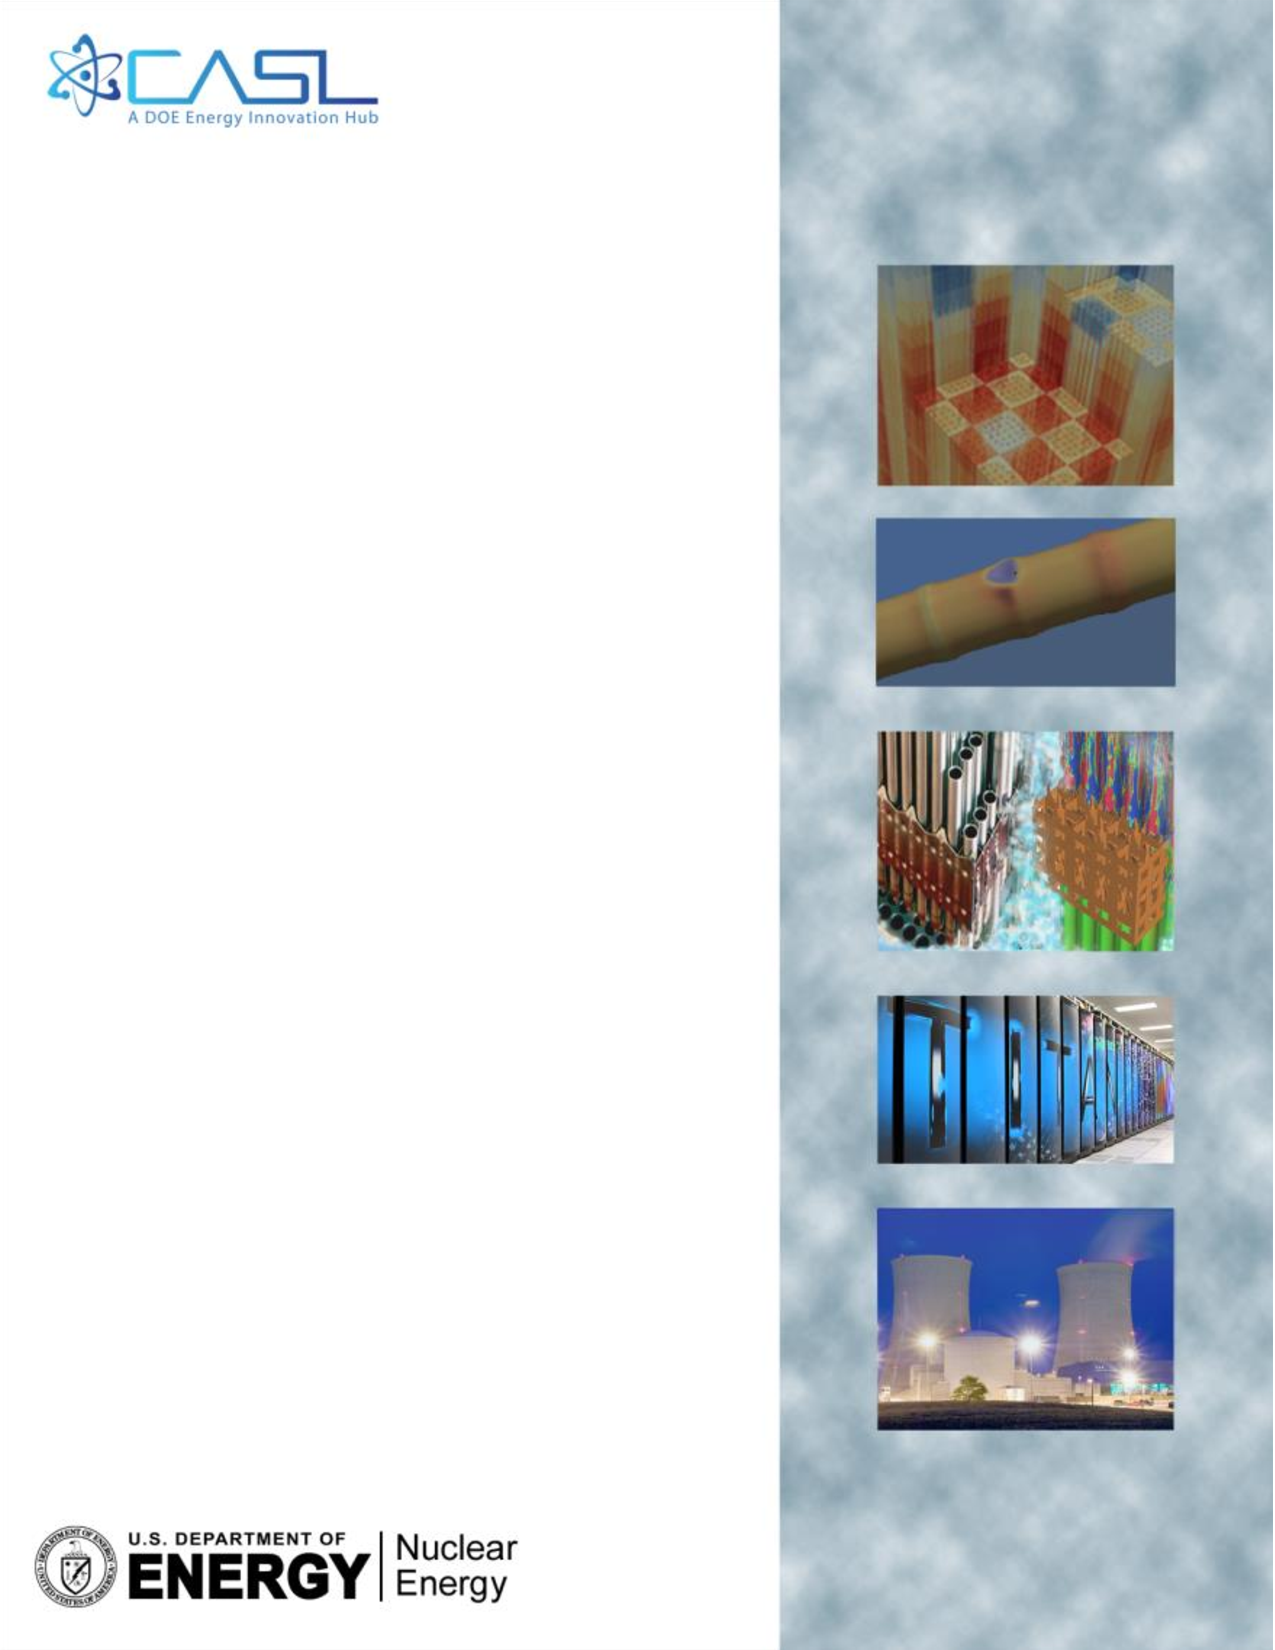
\includegraphics[width=\paperwidth,height=\paperheight]{template/casl_background.pdf}
  }%
}

% Define command to surround text in angle brackets
\newcommand{\brackets}[1]{\textlangle{}#1\textrangle{}}

% For formatting code
\newcommand{\codeblock}[1]{\texttt{#1}}

%increase space after captions
\setlength{\belowcaptionskip}{2pt}

% No indenting at start of paragraph
\setlength{\parindent}{0pt}

%increase space between paragraphs
\parskip 1em

\titleformat{\chapter}{\Huge\bfseries}{\thechapter. }{0pt}{\Huge\bfseries}

% set the section numbering depth and TOC depth
\setcounter{secnumdepth}{3}
\setcounter{tocdepth}{3}

% Use continuous counting scheme for floats
\counterwithout{table}{chapter}

\let\DeclareUSUnit\DeclareSIUnit
\let\US\SI
\DeclareUSUnit\F{F}
\DeclareUSUnit\ft{ft}
\DeclareSIUnit\inch{in}

%define the degree command for using temperature units
\providecommand{\degree}{\ensuremath{^{\circ}}}

% define new command to make custom vector notation
\newcommand{\vect}[1]{\vec{#1}}

% define a command to correct subscript size
\newcommand{\smallsub}[1]{\scriptscriptstyle{\text{#1}}}

% Define a macro to make the "by" symbol 
\newcommand{\by}{\texorpdfstring{\ensuremath{\times}}{x}}

% define command for quick scientific notation
\providecommand{\e}[1]{\ensuremath{\cdot10^{#1}}}